\documentclass[../../compsys.tex]{subfiles}
\begin{document}
\chapter{L11 - DNS \& P2P}
\vfill

\section{Global Process Naming and Addressing}
Every process communicating over the Internet is uniquely identified by a combination of an IP address and a port number.
\begin{center}
    \texttt{172.67.2.106:443}
\end{center}
\begin{itemize}
    \item[-] \textbf{172.67.2.106}: IP address of a network interface.
    \item[-] \textbf{443}: Port number (details below).
\end{itemize}
\subsection{Network Interfaces}
A network interface connects an end-system (such as a computer or smart device) to a network.  
\begin{itemize}
    \item[-] Each end-system has at least one network interface.
    \item[-] Each network interface has at least one unique IP address.
    \item[-] Examples: Your laptop's network card, or your car's onboard Wi-Fi.
\end{itemize}

\newpage
\subsection{Port Numbers}
Port numbers identify specific processes within a local system.
\begin{itemize}
    \item[-] Each process using network communication is assigned a unique port number.
    \item[-] On a server, port numbers for certain applications are restricted and standardized.
\end{itemize}

\subsubsection{Reserved Port Numbers}
Some port numbers are universally reserved for well-known services.
\begin{itemize}
    \item[-] Reserved ports are used exclusively by specific server processes.
    \item[-] Client processes and other servers should not use these reserved ports.
    \item[-] Examples: Ports 80, 8080, 443, and 8443 are reserved for web servers.
\end{itemize}

\subsection{Web Server Port Numbers}
Web servers use standardized ports for HTTP and HTTPS communication:
\begin{itemize}
    \item[-] \textbf{80, 8080}: HTTP (standard web traffic)
    \item[-] \textbf{443, 8443}: HTTPS (secure web traffic)
\end{itemize}
\textit{Note: HTTPS is the encrypted, secure version of HTTP.}
\subsection{The Domain Name System (DNS)}
DNS is an essential Internet system that translates human-friendly domain names into IP addresses.

\subsubsection{Example}
When you enter a URL such as:
\begin{itemize}
    \item \textbf{https://www.epfl.ch/labs/nal/publications}
    \item \textbf{www.epfl.ch}: Hostname (DNS name)
    \item \textbf{labs/nal/publications}: Path to the resource
\end{itemize}

\noindent The Domain Name System (DNS) maps domain names like \texttt{www.epfl.ch} to IP addresses (e.g., \texttt{128.178.211.3}). This translation allows users to access network interfaces by name rather than by numeric address, making the Internet more user-friendly and scalable.

\subsubsection{DNS Translation in Action}
\begin{enumerate}
    \item The web client reads the URL and identifies the protocol: \textbf{https}.
    \item For HTTPS, the default port number is \textbf{443} (or sometimes 8443).
    \item The web client extracts the DNS name (\texttt{www.epfl.ch}) and sends a DNS query to obtain its IP address.
    \item Once resolved, it can contact the web server process at \texttt{128.178.211.3:443}.
\end{enumerate}

\subsection{Application Design}
The design of a distributed application requires answering:
\begin{itemize}
    \item[-] How many processes/threads are involved, and their roles.
    \item[-] What communication protocols are used between them.
\end{itemize}
For DNS, this means defining client and server roles and their communication.

\subsection{How Does DNS Work?}
DNS uses a client-server architecture with specialized processes:

\begin{itemize}
    \item[-] When you type a URL, your web client extracts the DNS name (e.g., \texttt{www.epfl.ch}).
    \item[-] A local process, called the \textbf{DNS client} or \textbf{stub resolver}, creates a DNS query.
    \item[-] The DNS client sends this query to a \textbf{local DNS server} (resolver), typically nearby.
    \item[-] The DNS server process listens on port 53 and replies with the IP address.
    \item[-] The DNS client relays the response back to the web client.
    \item[-] The web client can now communicate with the web server using the IP address and correct port.
\end{itemize}

\begin{center}
    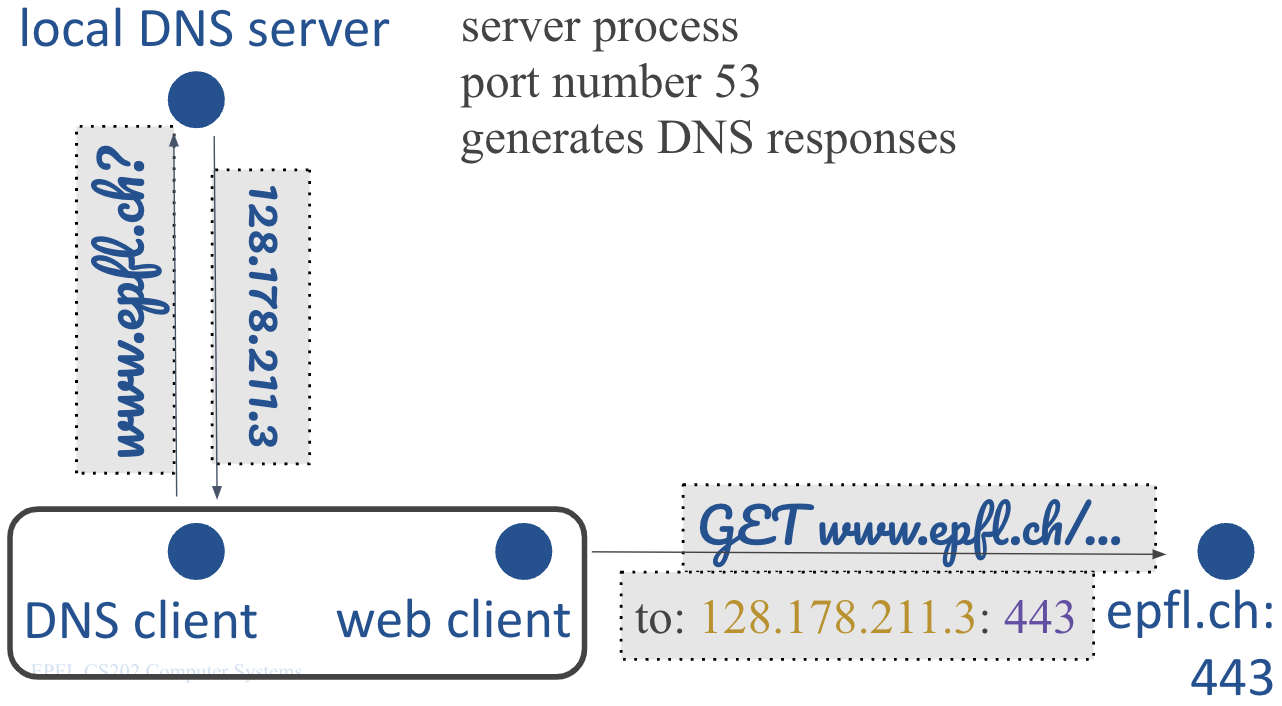
\includegraphics[width=0.5\textwidth]{images/dns.png}
\end{center}

\subsubsection{Why Not a Single DNS Server?}
A single-server DNS design would not scale:
\begin{itemize}
    \item[-] It would be overloaded by global traffic.
    \item[-] It could not provide low latency to all clients.
    \item[-] It would be a single point of failure.
    \item[-] Maintenance would be unmanageable at Internet scale.
\end{itemize}

\subsection{Scalability}
Scalability is the ability of a system to grow while maintaining good performance and reasonable cost, independently from size.
\subsection{Distributed DNS}
The Domain Name System (DNS) is not managed by a single server, but as a distributed, hierarchical system. This structure ensures scalability, reliability, and high performance for name resolution on the Internet.

\begin{center}
    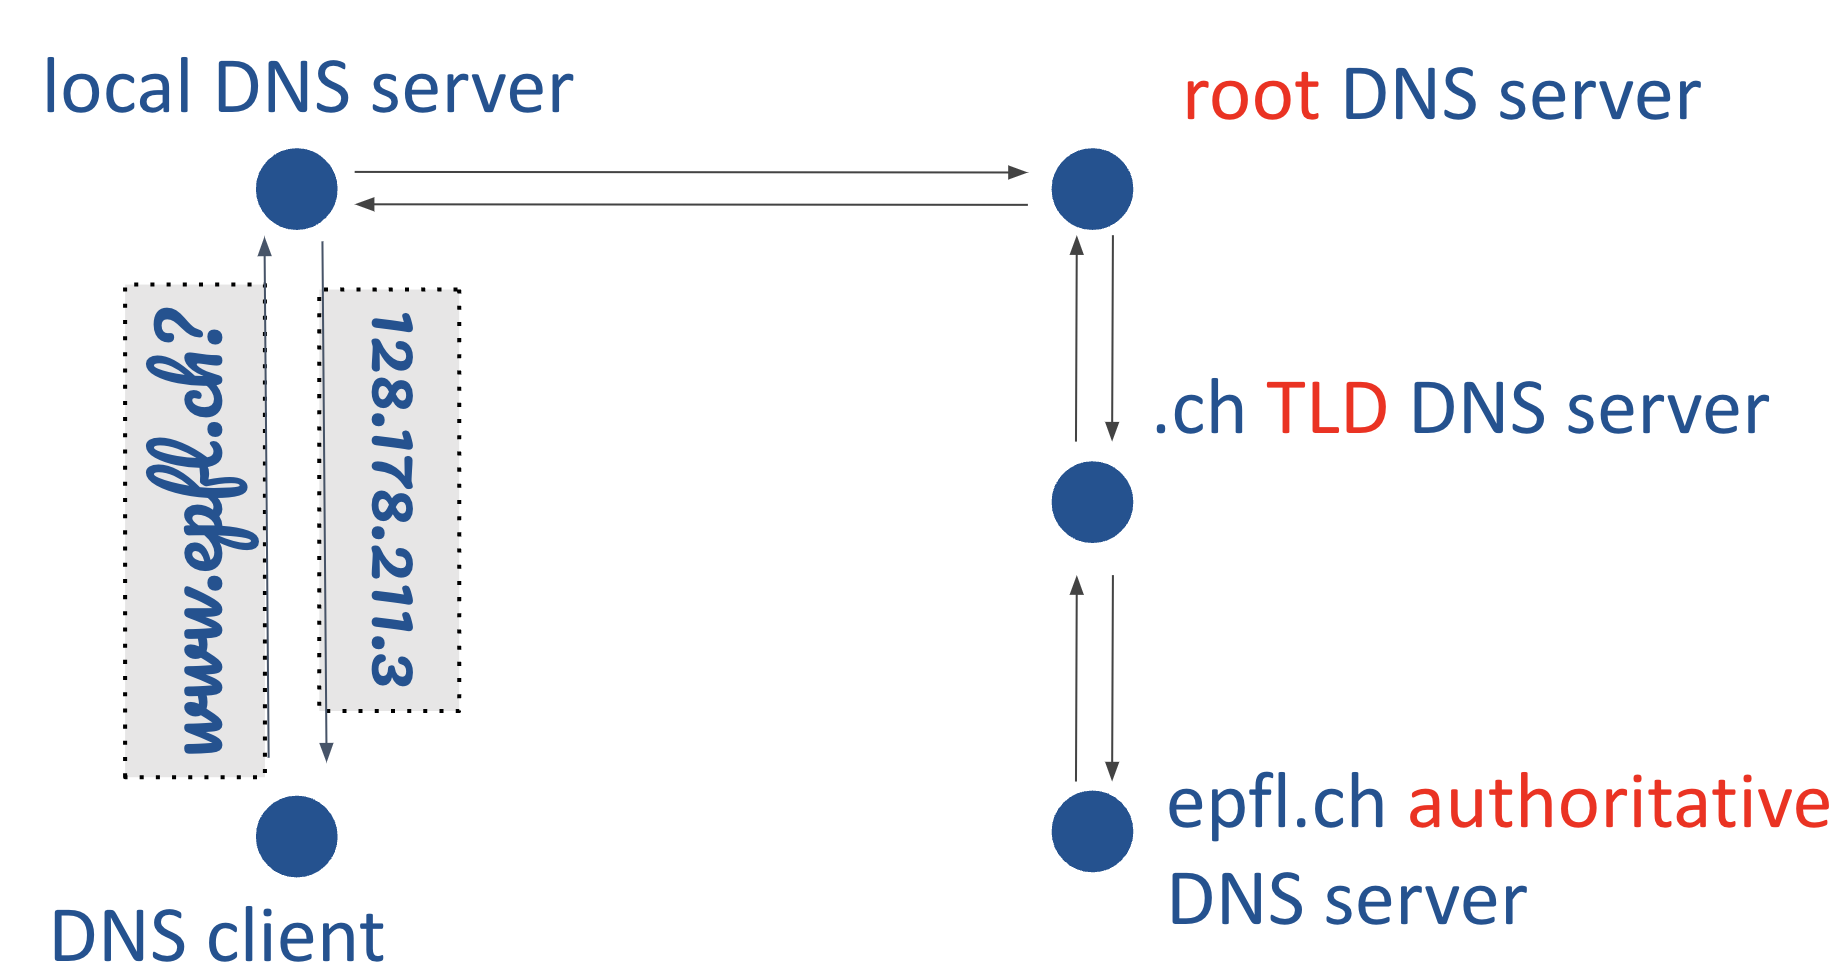
\includegraphics[width=0.5\textwidth]{images/translation.png}
\end{center}

When a DNS client wants to resolve a domain such as \texttt{epfl.ch}, the following process occurs:
\begin{itemize}
    \item The client queries its local DNS server.
    \item If the local server does not know the answer, it queries a \textbf{root DNS server}.
    \item If the root server does not know the answer, it forwards the query to a \textbf{TLD (Top-Level Domain) server} (e.g., for \texttt{.ch}).
    \item If the TLD server does not know, it asks the \textbf{authoritative DNS server} for the specific domain (e.g., \texttt{epfl.ch}).
    \item The authoritative DNS server provides the definitive answer for the requested domain.
\end{itemize}

\subsubsection{DNS Hierarchy}
DNS servers are organized hierarchically to efficiently manage and resolve domain names. At each level, servers have specific responsibilities.

\begin{center}
    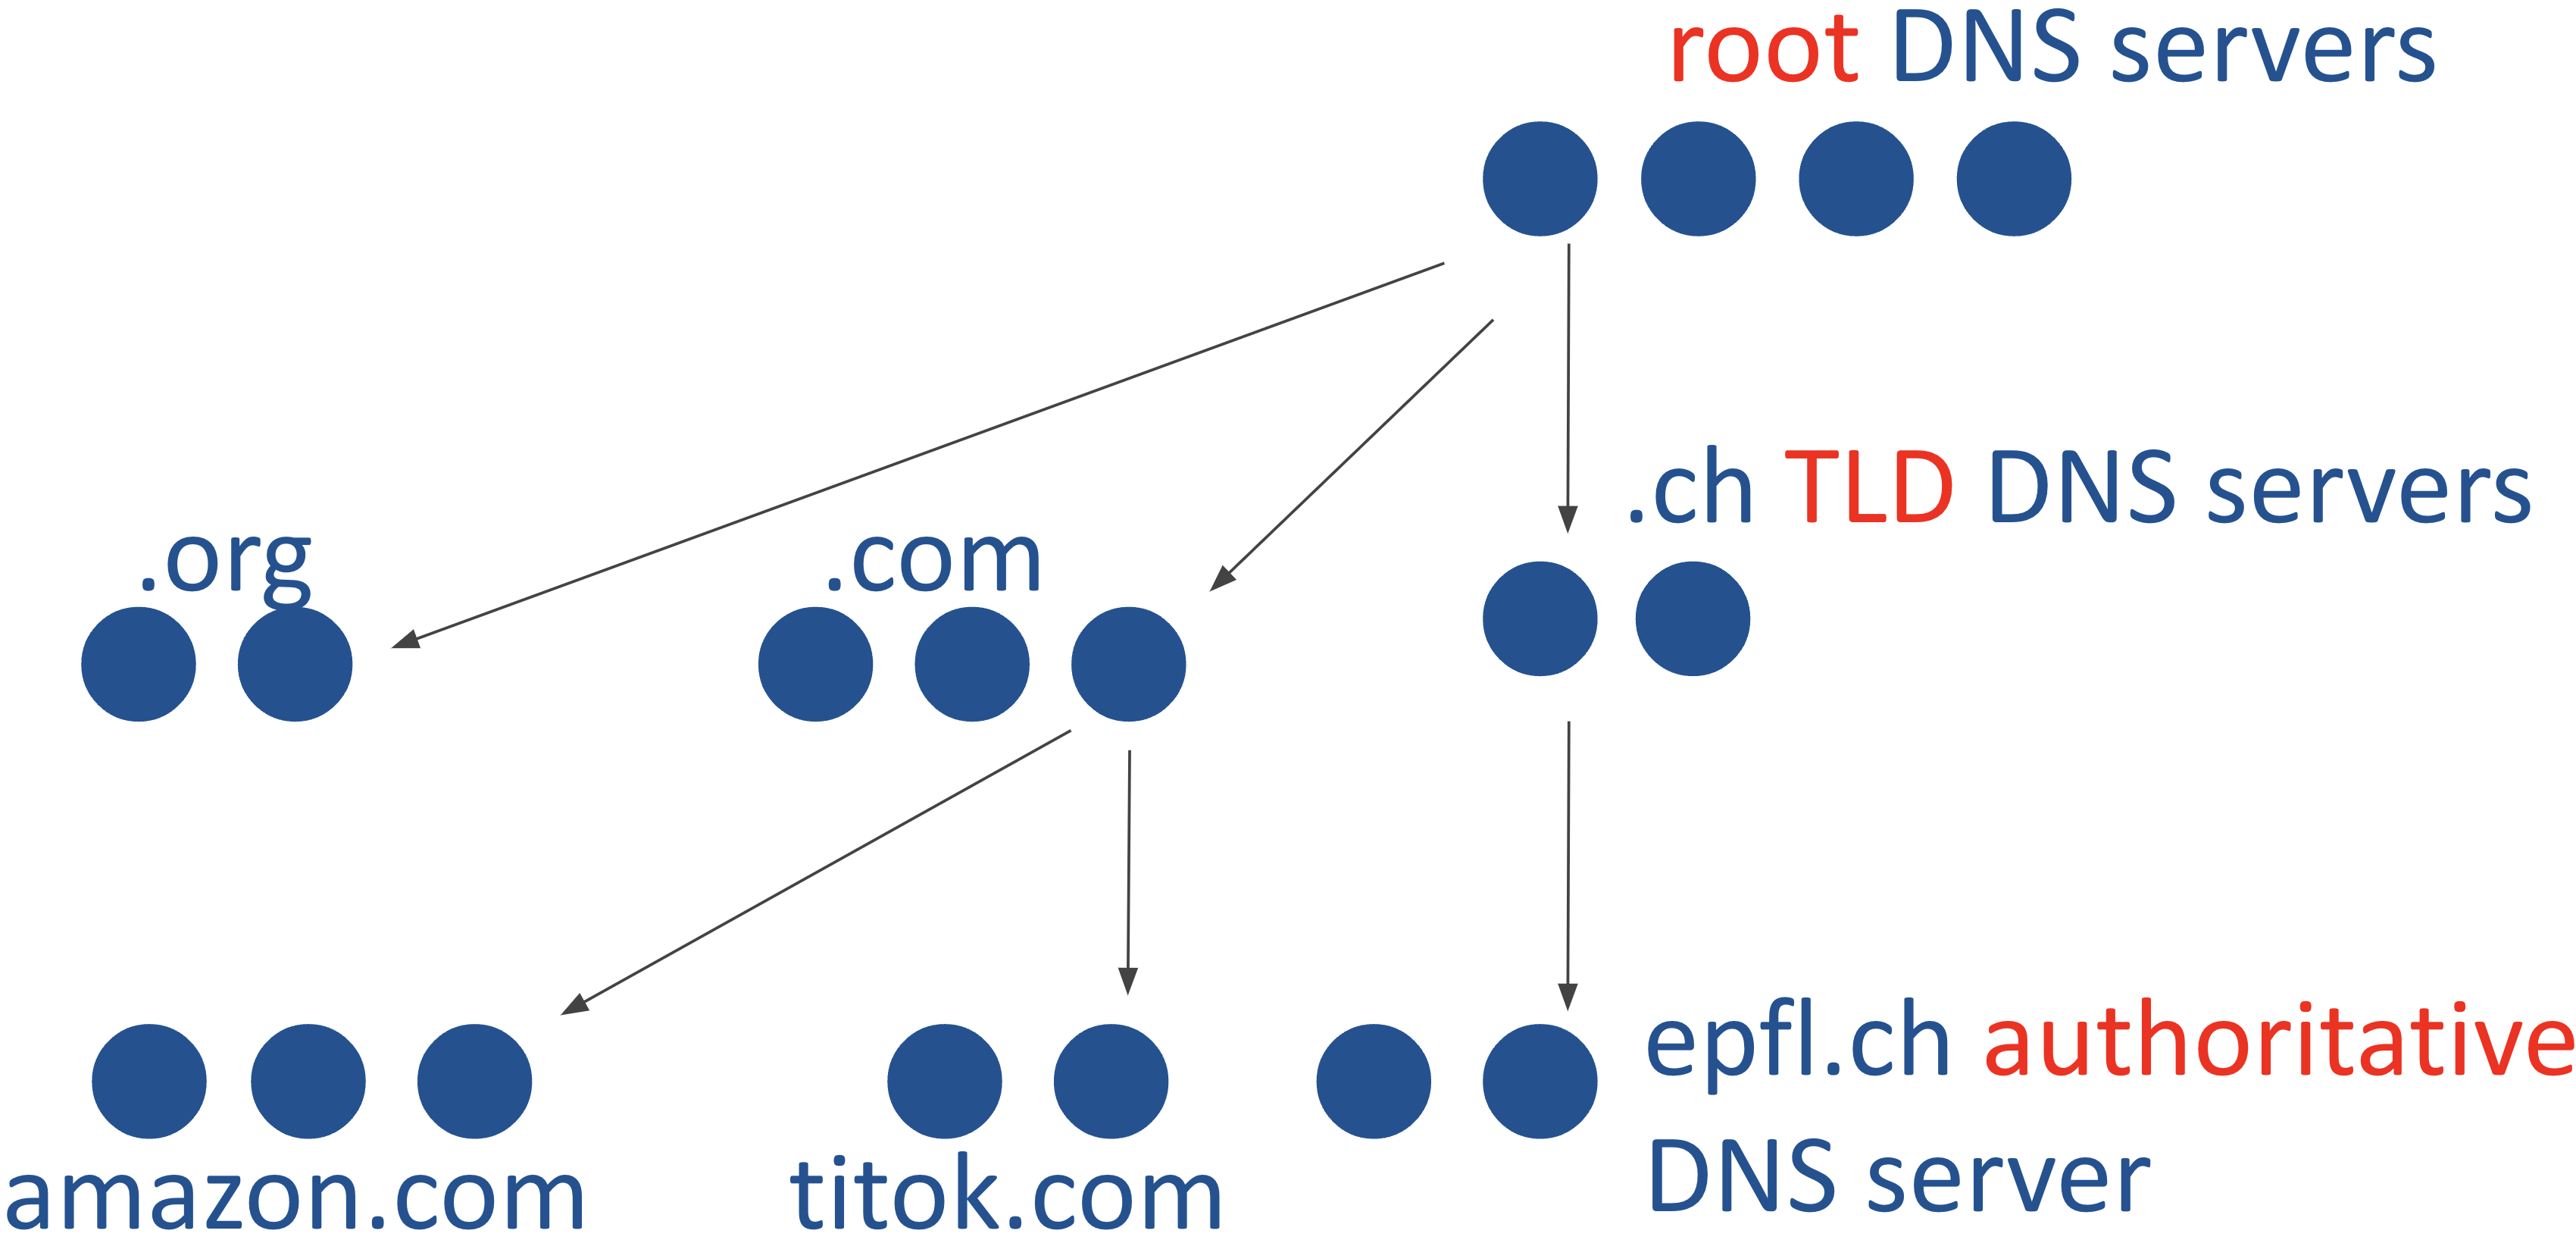
\includegraphics[width=0.5\textwidth]{images/hiearchy.png}
\end{center}

\begin{itemize}
    \item \textbf{Root DNS servers} are at the top of the hierarchy. They know how to reach all TLD servers.
    \item \textbf{TLD DNS servers} manage domains for top-level domains (e.g., \texttt{.ch}, \texttt{.com}, \texttt{.org}). They know the authoritative servers for all second-level domains under their TLD.
    \item \textbf{Authoritative DNS servers} hold the final, definitive information about their specific domain (e.g., \texttt{epfl.ch}, \texttt{ricardo.ch}). They know the IP addresses for all hostnames in their domain.
\end{itemize}

For example, an authoritative server for \texttt{epfl.ch} knows the addresses of all hosts ending with \texttt{epfl.ch}. Similarly, a TLD server for \texttt{.ch} knows how to reach authoritative servers for all \texttt{.ch} domains.

\subsection{DNS Query Resolution}
There are two main approaches for a DNS query to reach a server that can answer it. Each approach offers different trade-offs in terms of efficiency and server workload.

\subsubsection{Recursive Query}
In a \textbf{recursive query}, the client asks a DNS server to resolve the name entirely. The server takes responsibility for querying other DNS servers until it obtains the answer, which it then returns to the client.

\begin{center}
    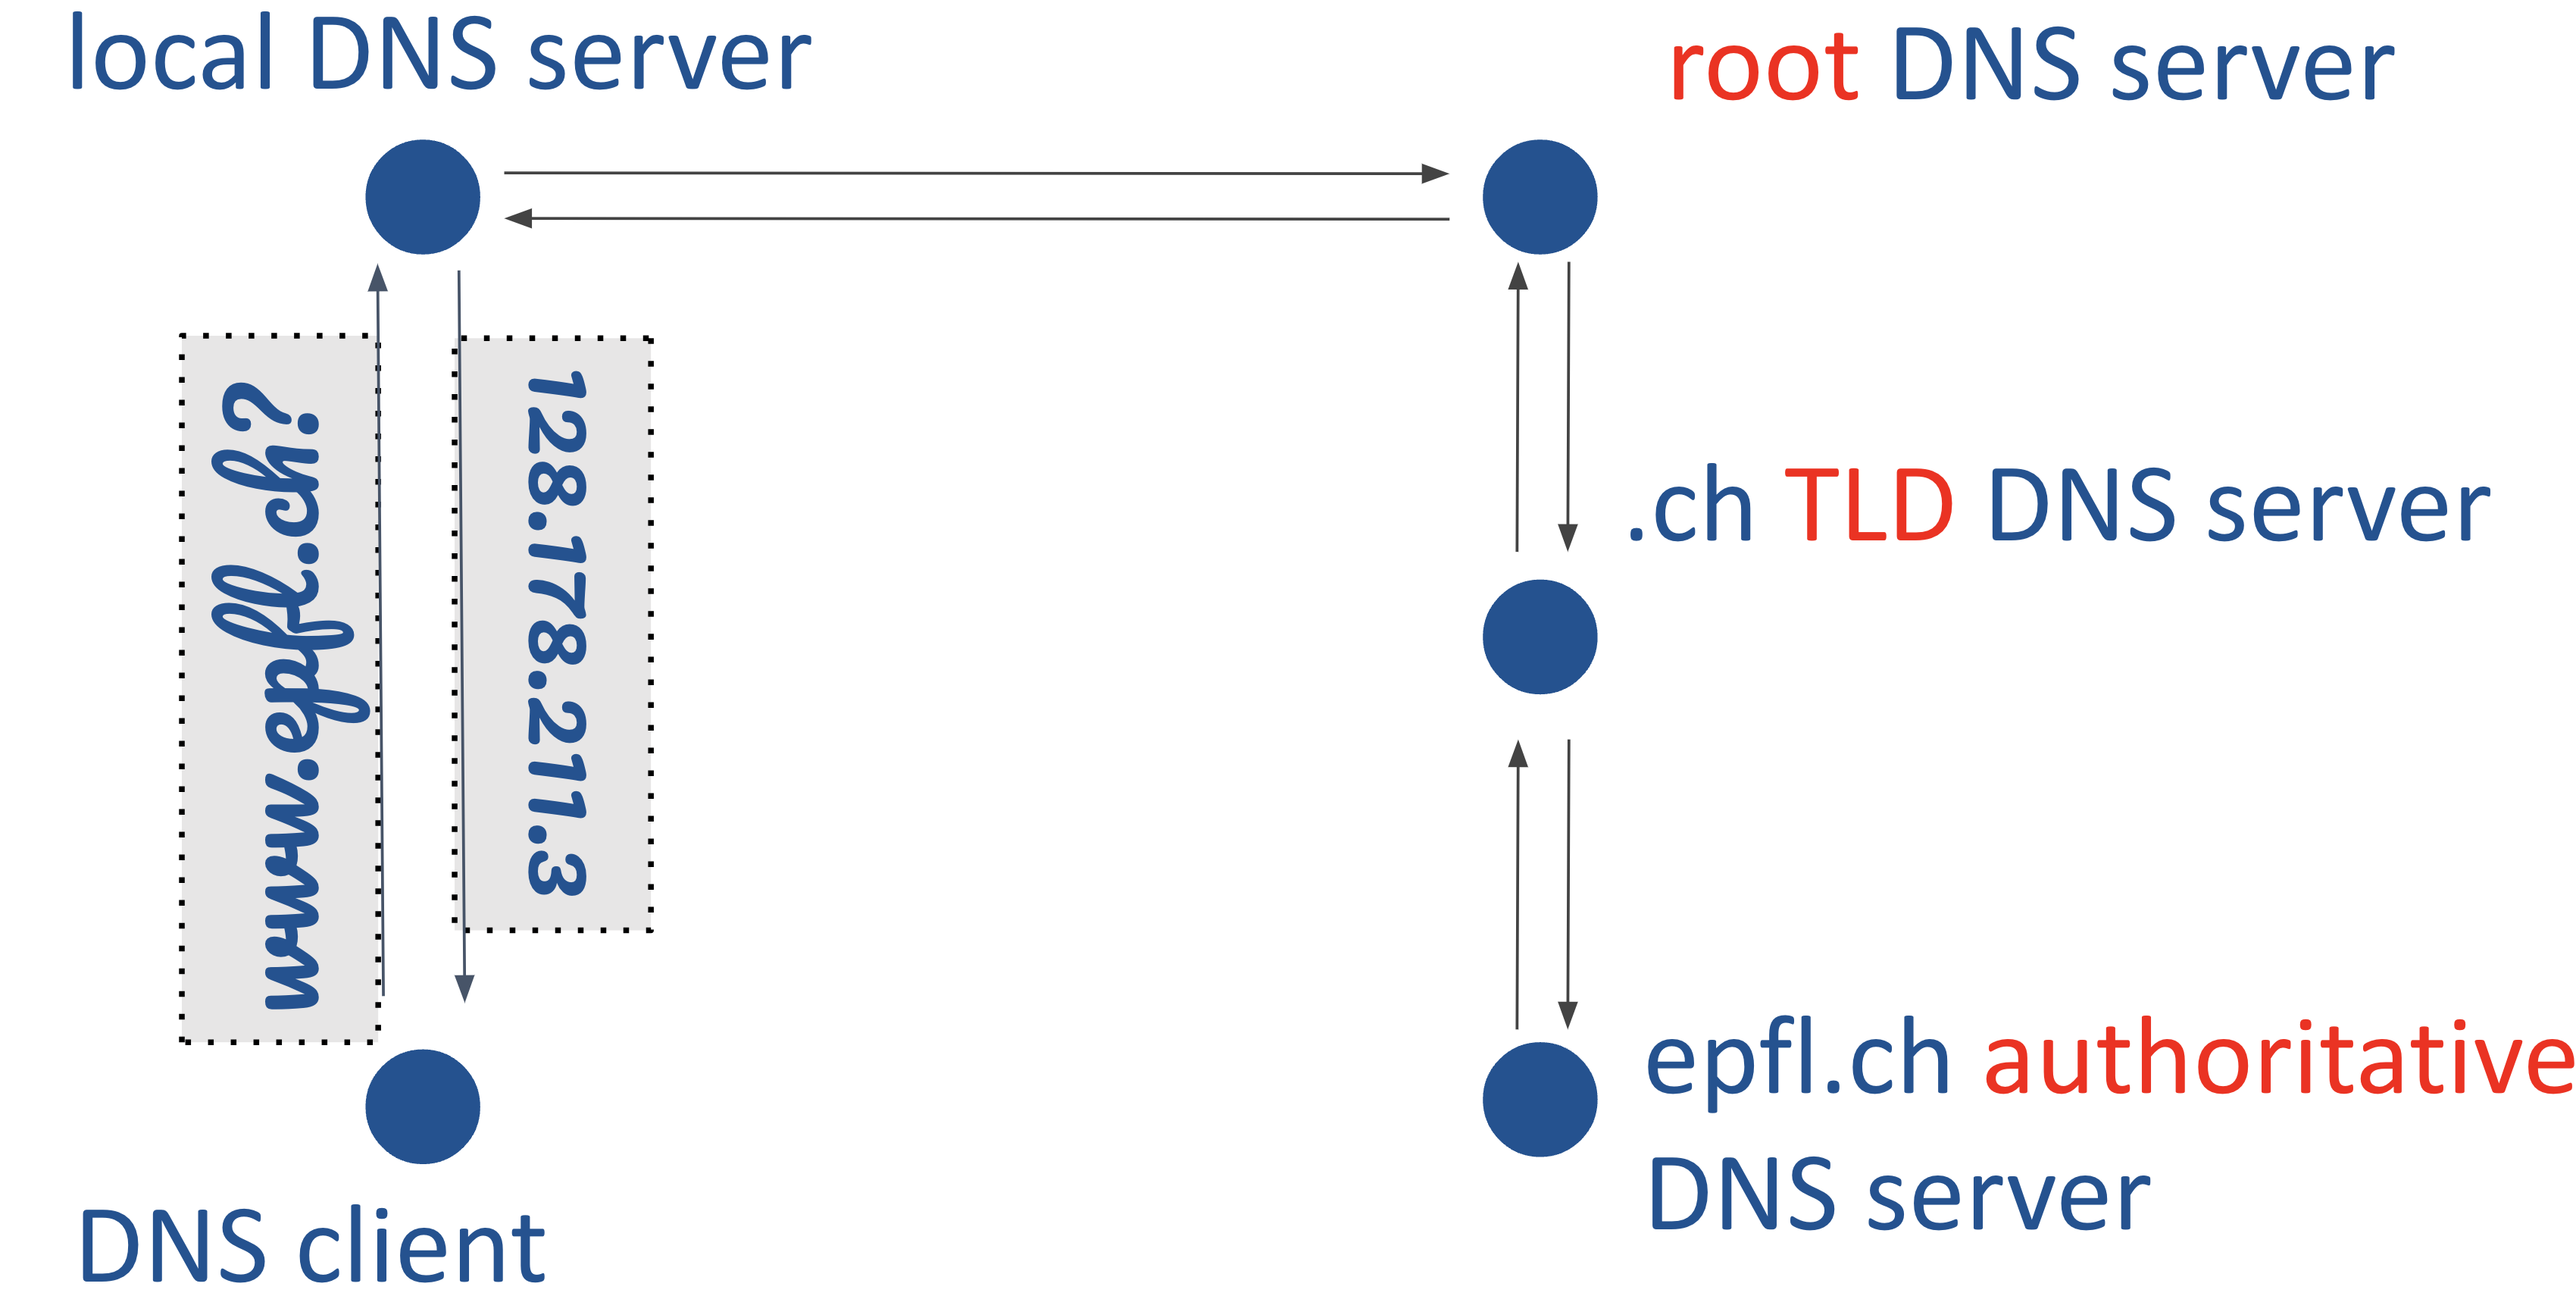
\includegraphics[width=0.5\textwidth]{images/recursive.png}
\end{center}

\begin{itemize}
    \item[-] Every DNS client knows at least one local DNS server.
    \item[-] Every DNS server knows at least one root DNS server.
    \item[-] Each root DNS server knows at least one TLD DNS server per TLD.
    \item[-] Each TLD DNS server knows at least one authoritative DNS server for each second-level domain it manages.
\end{itemize}
If the hierarchy works correctly, every DNS query should eventually receive a response.

\subsubsection{Iterative Query}
In an \textbf{iterative query}, a DNS server responds to the client with the address of the next server to contact if it cannot answer directly. The client then queries that server, repeating the process until it finds the authoritative answer.

\begin{center}
    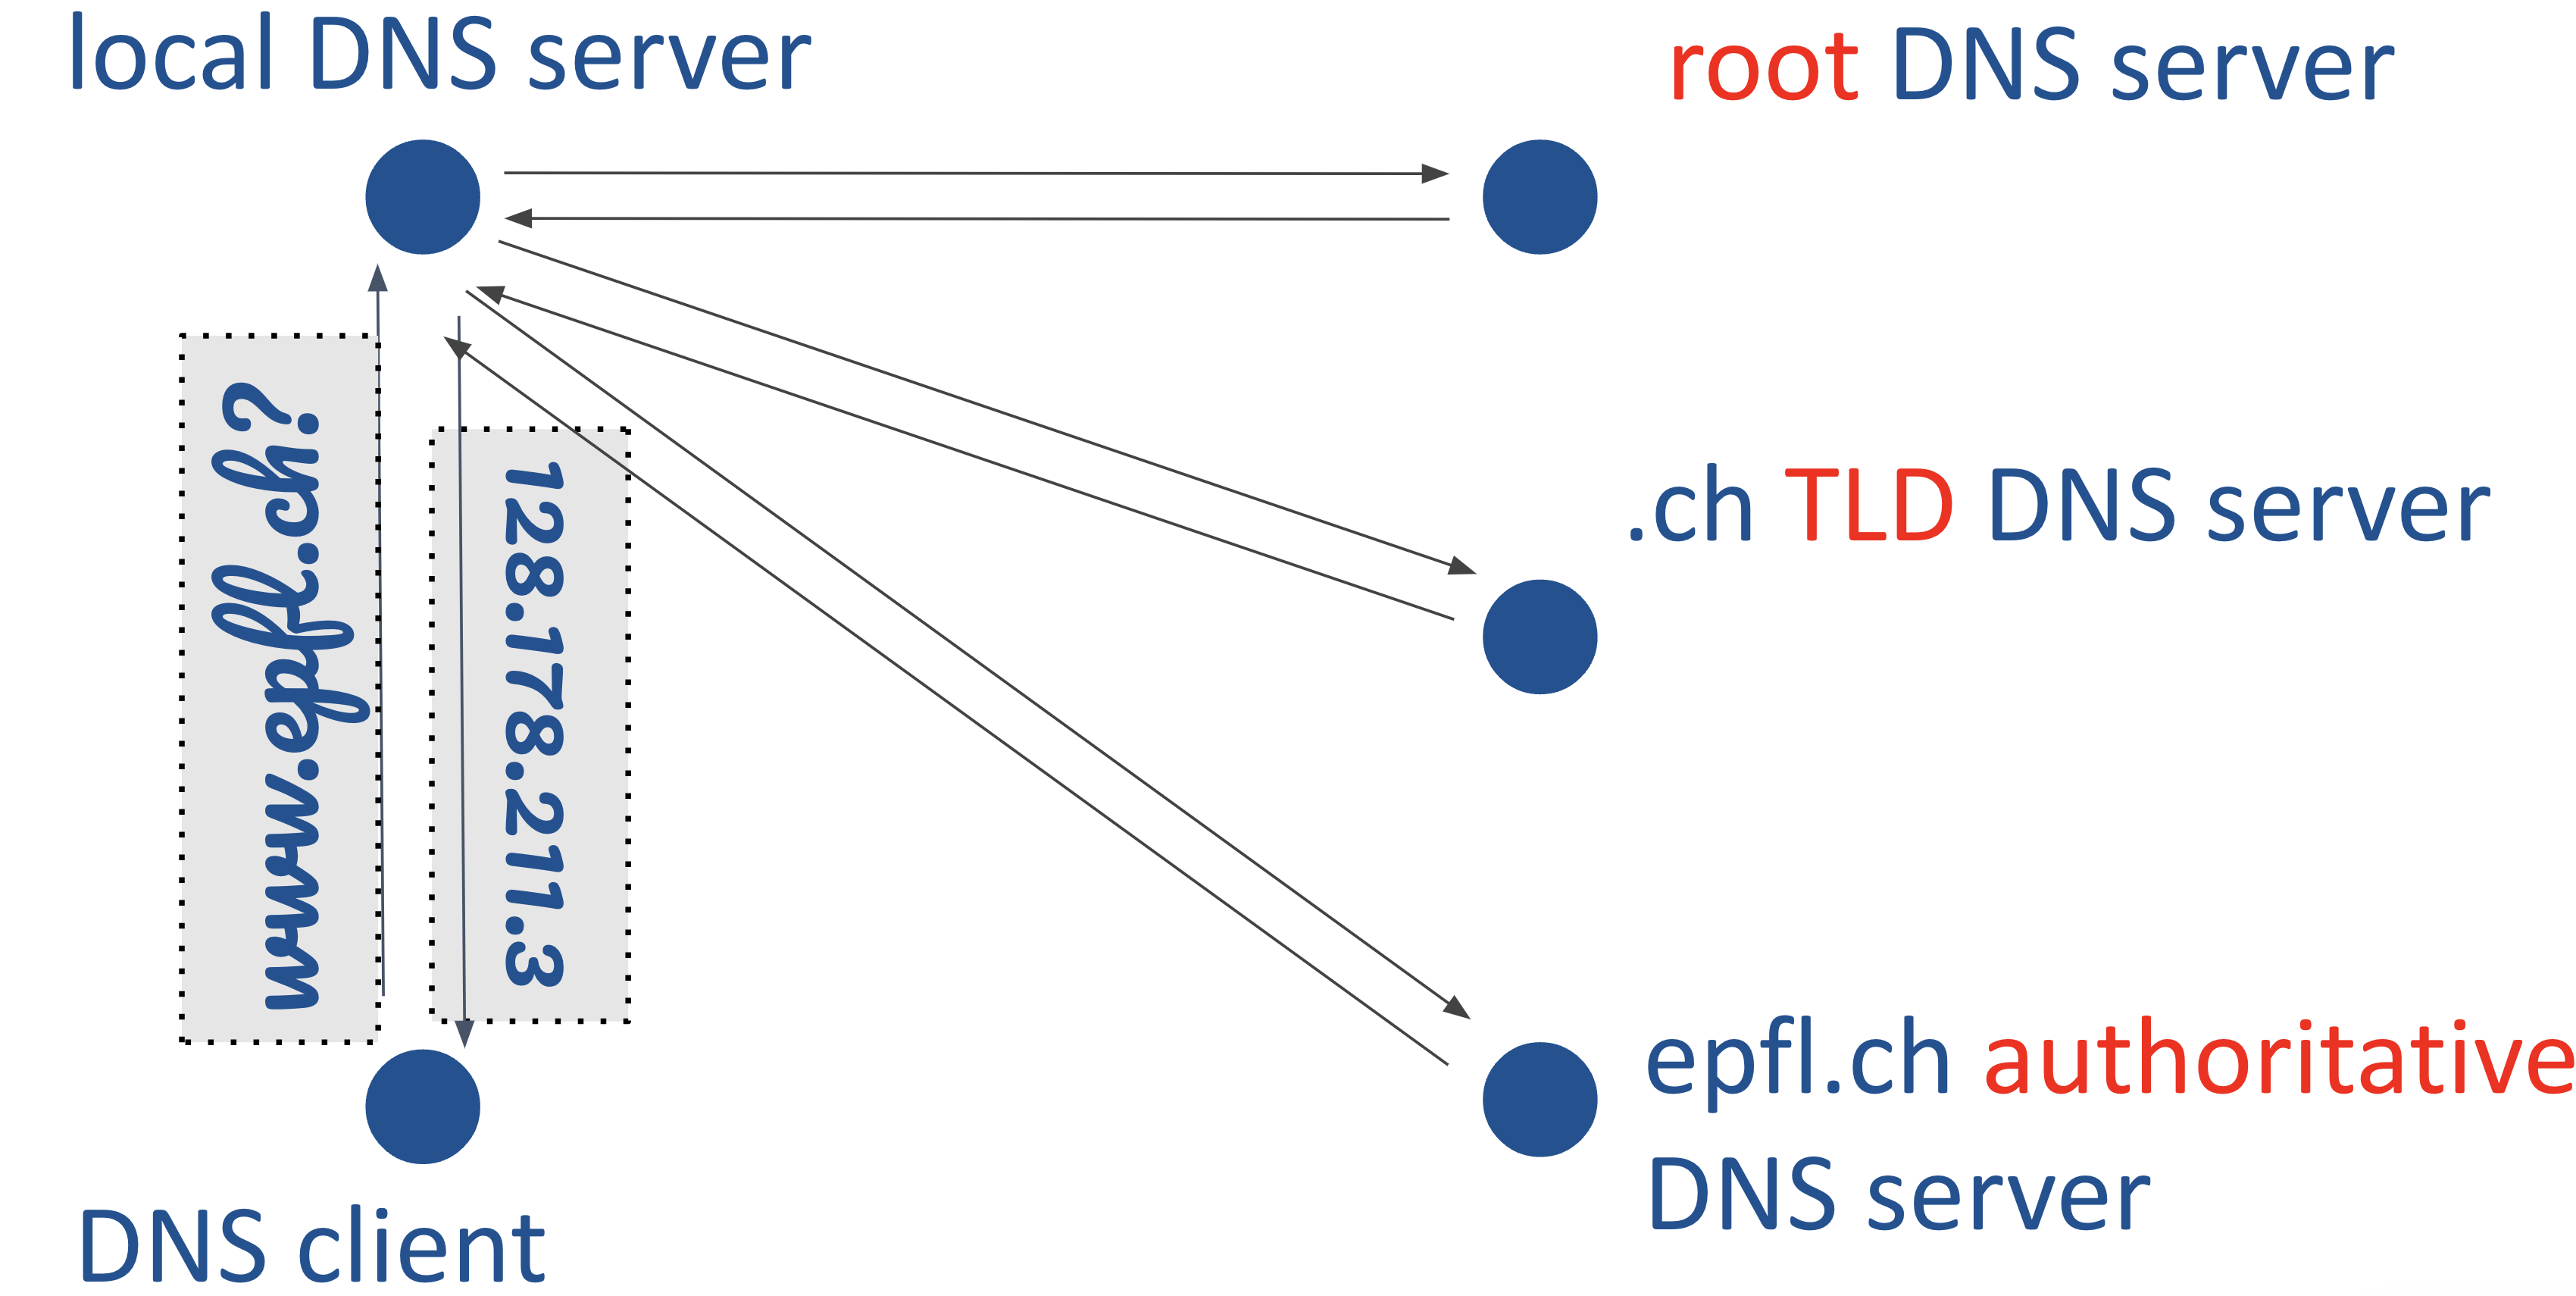
\includegraphics[width=0.5\textwidth]{images/iterative.png}
\end{center}
This model is common in practice, often as a mix of recursive and iterative queries: the local DNS server handles recursion for the client, while upstream servers use iteration.

\subsubsection{Benefits of the Hierarchy}
This hierarchical structure significantly improves DNS scalability:
\begin{itemize}
    \item[-] No DNS server needs to know all domain names worldwide.
    \item[-] Each server only needs to know where to find the next more specific server.
\end{itemize}

\noindent
\subsubsection{DNS Caching}
DNS queries can involve multiple servers, which may introduce noticeable delays. To improve performance, DNS extensively uses \textbf{caching}. 

\textit{Caching} allows both DNS clients and servers to store recent DNS query results, so repeated requests for the same domain name can be answered much faster without contacting other servers.

The primary challenge of caching is ensuring the data remains up-to-date. Each DNS response includes a \textbf{Time To Live (TTL)}, which specifies the maximum time the result should be cached. When the authoritative server sends a response, it sets an initial TTL. As the response is passed along the DNS hierarchy, each server reduces the TTL by the elapsed time before forwarding or serving the cached result.

\begin{center}
    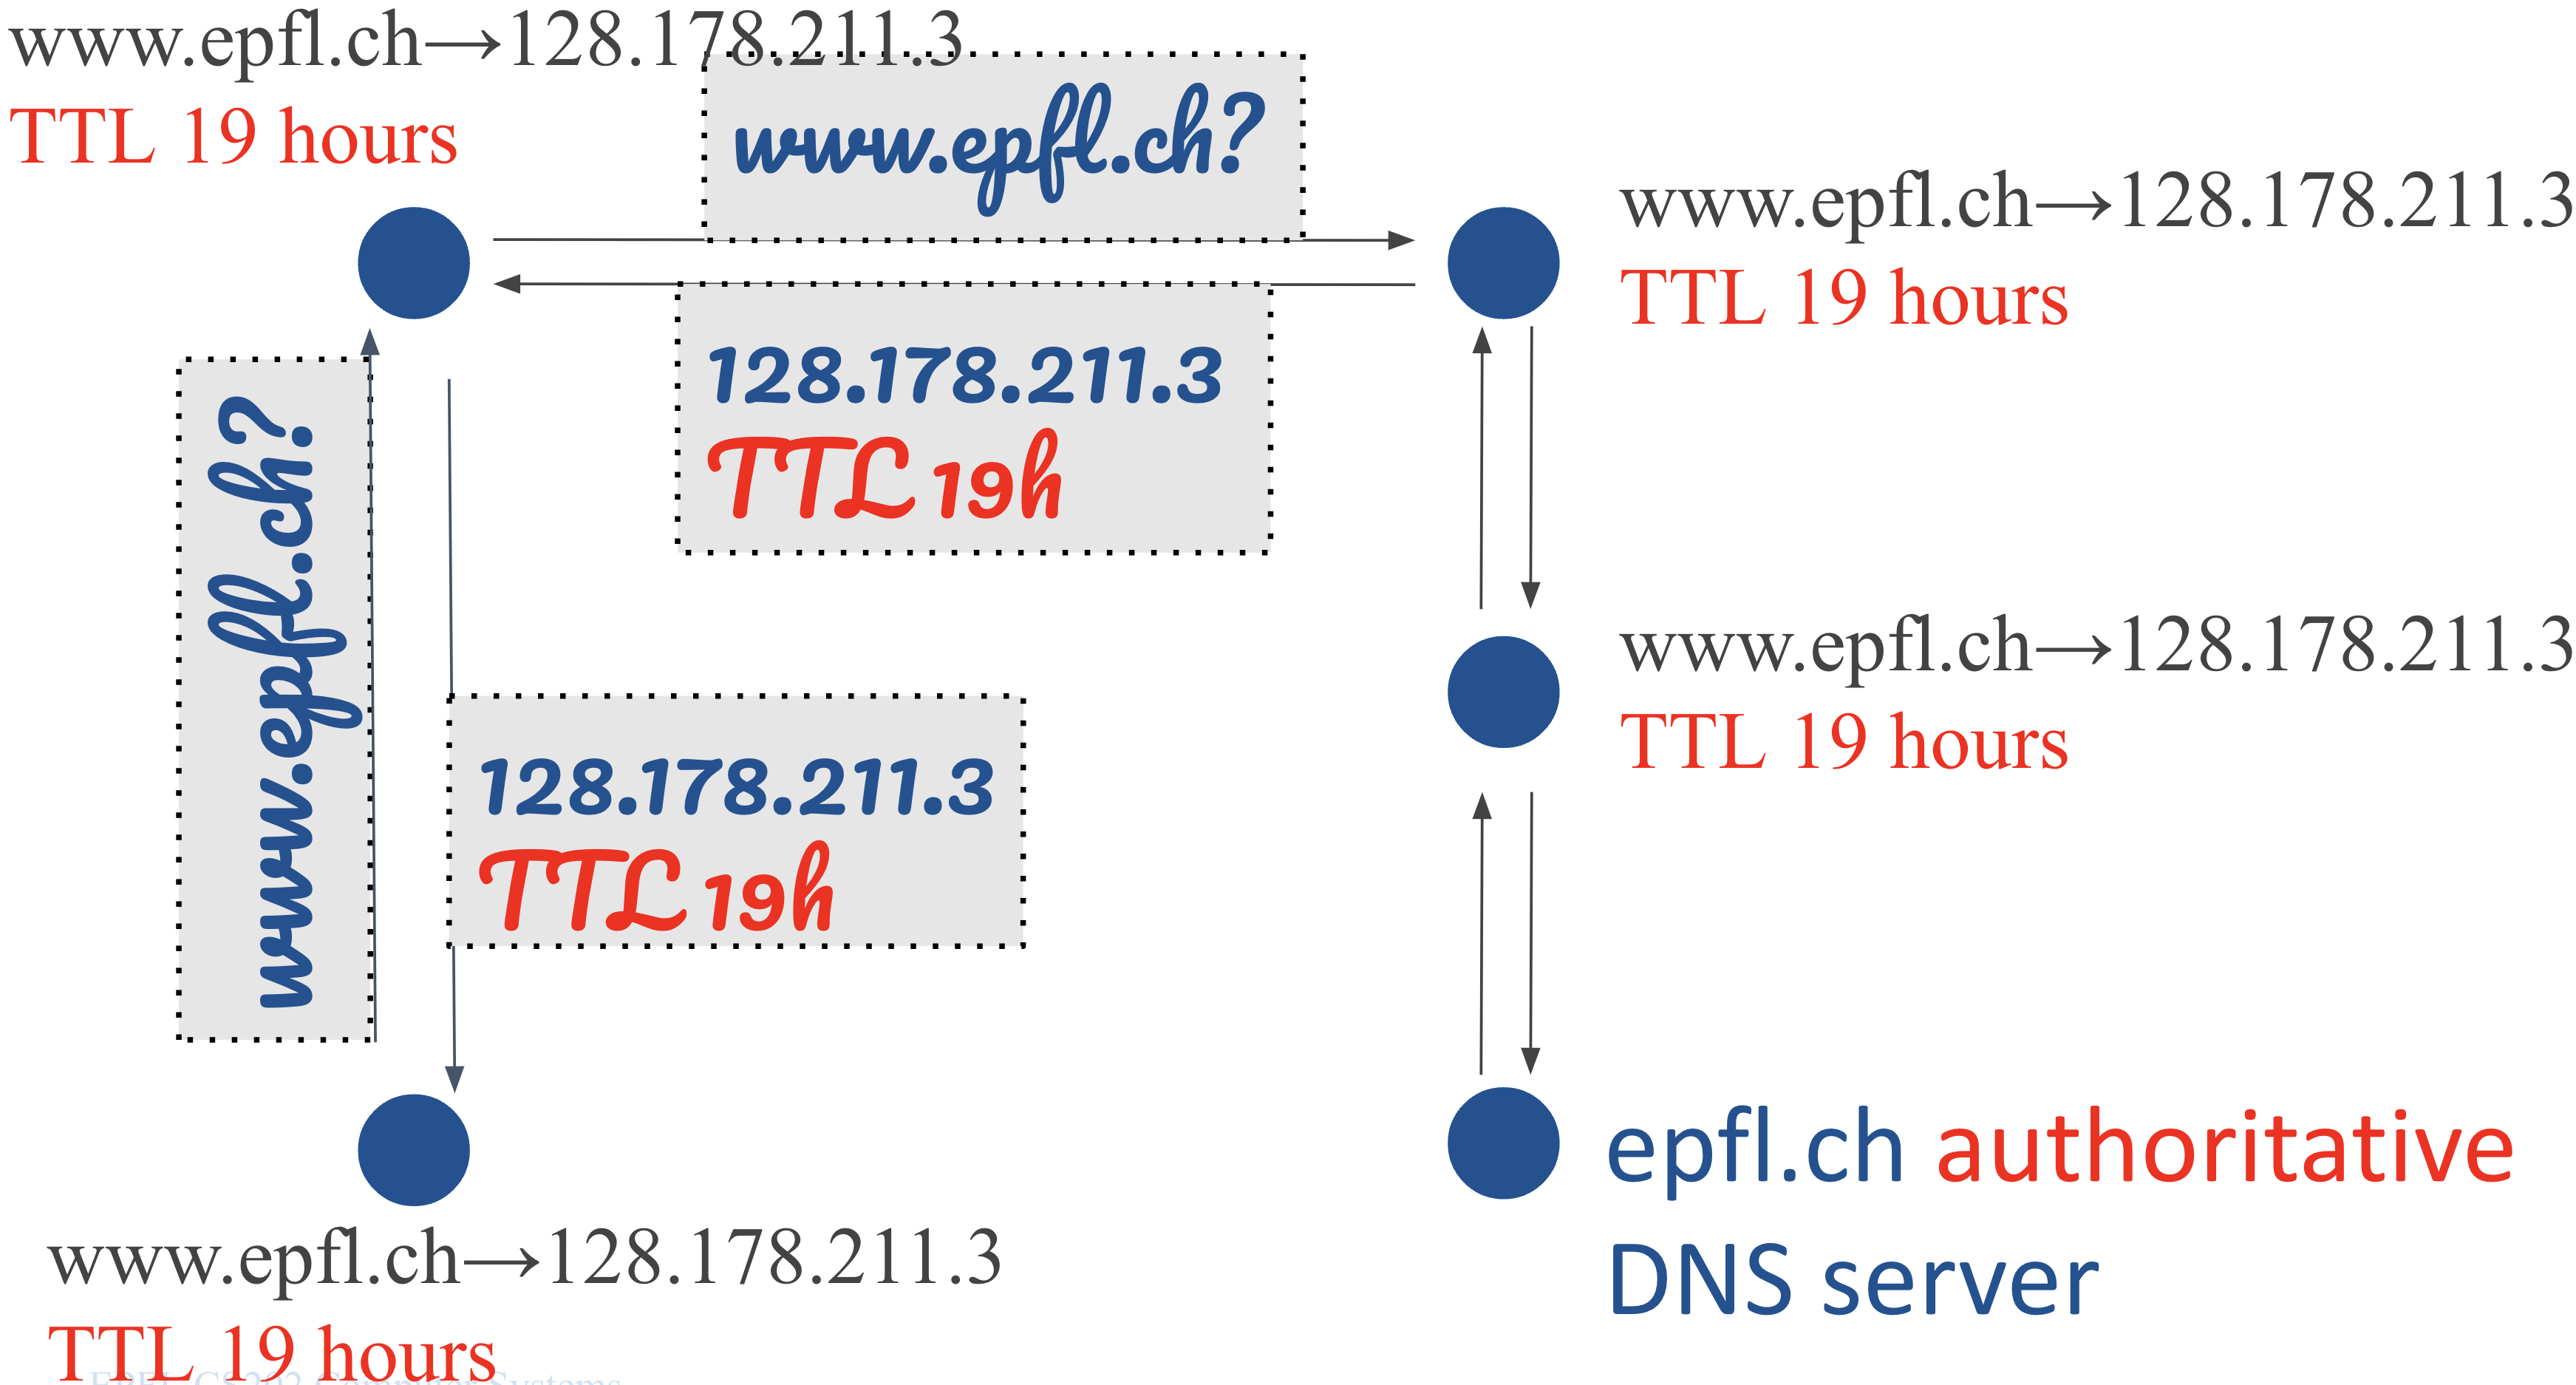
\includegraphics[width=0.6\textwidth]{images/ttl.png}
\end{center}

\textit{Example:}
\begin{itemize}
    \item[-] The authoritative server for \texttt{epfl.ch} responds with a TTL of 24 hours.
    \item[-] After 4 hours, a TLD server responds with a TTL of 20 hours.
    \item[-] After another hour, a root server responds with a TTL of 19 hours, and so on.
    \item[-] Each caching server and client will use the remaining TTL value.
\end{itemize}

\subsubsection{DNS Processes}
DNS operates through a combination of queries and responses, with the help of a distributed hierarchy:
\begin{itemize}
    \item The \textbf{DNS client} generates queries to resolve domain names.
    \item The \textbf{local DNS server} (also called a resolver) processes client requests and can respond directly from cache or contact higher-level servers.
    \item The \textbf{hierarchy of DNS servers} assists in generating accurate responses for the client.
\end{itemize}

\subsubsection{DNS Hierarchy: Summary}
The DNS hierarchy consists of three main layers:
\begin{itemize}
    \item[-] \textbf{Root servers} (top): Know how to reach all TLD servers.
    \item[-] \textbf{Top-level domain (TLD) servers} (middle): Responsible for specific TLDs (e.g., \texttt{.ch}, \texttt{.com}), know authoritative servers for each second-level domain.
    \item[-] \textbf{Authoritative servers} (bottom): Responsible for a specific domain (e.g., \texttt{epfl.ch}), and know all hostnames within that domain.
\end{itemize}

\subsubsection{DNS Protocol}
DNS communication is based on a simple query-response protocol:
\begin{itemize}
    \item A \textbf{query} (or request) is sent from a client or server to another DNS server to obtain information about a domain name.
    \item A \textbf{response} contains the answer, provided as a list of \textit{resource records} (RRs).
\end{itemize}

A \textbf{resource record (RR)} is a data structure containing specific DNS information. There are several common types:
\begin{itemize}
    \item[-] \textbf{A record:} Maps a DNS name to an IPv4 address.
    \item[-] \textbf{AAAA record:} Maps a DNS name to an IPv6 address.
    \item[-] \textbf{CNAME record:} Maps a DNS name to another DNS name (alias).
    \item[-] \textbf{MX record:} Specifies the mail server for a domain.
    \item[-] \textbf{SOA record:} Indicates the Start of Authority for a domain.
\end{itemize}

\textit{Prof. Note:} You do not need to memorize all types, but it is useful to know the main examples and their purpose.
\end{document}